\section{Architecture logicielle}
\label{sec:architecture}

\noindent
Cette section décrit l'organisation interne du compilateur \texttt{decac} et les principales interactions entre les classes qui l'implémentent.

\subsection{Vue d'ensemble}
\noindent
Le compilateur est organisé en trois étapes principales correspondant aux phases de compilation :

\begin{itemize}[label=$\circ$]
    \item Étape A : Analyse lexicale et syntaxique $\to$ scinde le code source en token et construit l'abstrait (AST) et fait la correspondance entre les règles de la grammaire définies dans les fichiers \texttt{Lexer.g4} et \texttt{Parser.g4} et le paquetage \texttt{tree} à l'aide de \texttt{ANTLR}
    \item Étape B : Vérifications contextuelles $\to$ l'AST est parcouru afin de vérifier la validité sémantique du programme de décorer l'AST en conséquence
    \item Étape C : Génération de code $\to$ génère les instructions assembleur pour la machine \texttt{IMA}.
\end{itemize}

\noindent
Ces différentes phases sont implémentées dans des paquetages distincts et sont gérées par la classe \texttt{DecacCompiler}, appelée depuis le point d'entrée du compilateur. La figure~\ref{fig:pipeline} schématise les interactions entre les principaux composants.

\begin{figure}[H]
    \centering
    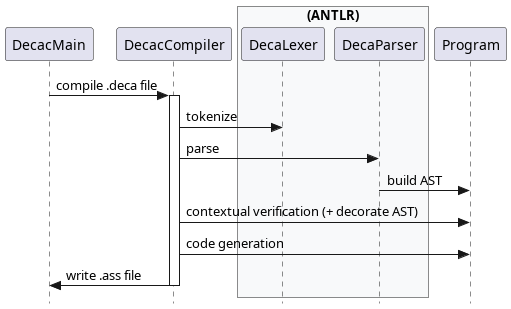
\includegraphics[width=0.8\textwidth]{diagrams/out/archi-pipeline.png}
    \caption{Vue d'ensemble de la chaîne de compilation}
    \label{fig:pipeline}
\end{figure}


La classe \texttt{DecacCompiler} joue un rôle central dans l'architecture du compilateur et coordonne l'exécution des différentes phases de compilation.


\subsection{Organisation générale des paquetages}
\noindent
Le code source est organisé autour de paquetages distincts : 
\begin{itemize}[label=$\circ$]
    \item \texttt{syntax} : classes (\texttt{AbstractDecaParser}, \texttt{AbstractDecaLexer})qui permettent de faire le lien entre le compilateur et les classes générées par \texttt{ANTLR} selon les règles écrites dans les fichiers .g4 + gestionnaires d'erreurs
    \item \texttt{tree} : classes permettant la représentation des nœuds de l'arbre abstrait
    \item \texttt{context} : toutes les classes (Types, Environnements, Définitions) utilisées lors de la décoration et vérification contextuelle + gestionnaire d'erreurs contextuelles (\texttt{ContextualError})
    \item \texttt{codegen} : gestionnaires de pile, registres, labels, table des méthodes, et erreurs à l'exécution
    \item \texttt{ima} : représentation des instructions assembleur IMA
    \item \texttt{tools} : classes utilitatires (table des symboles, affichage de l'AST, erreurs internes).
\end{itemize}


\subsection{Échange d'information entre les étapes : l'arbre syntaxique abstrait (AST)}
\label{subsec:ast-architecture}

\noindent
Les données générées par le compilateur sont transmises au travers de l'arbre syntaxique abstrait. Celui-ci est construit lors de l'analyse syntaxique, enrichi lors de l'analyse contextuelle (ajout d'informations de type et de définitions), puis parcouru lors de la génération de code. Chaque phase effectue un ou plusieurs parcours de l'arbre y ajoute des nœuds (\texttt{ConvFloat}) ou des informations supplémentaires (types, définitions) mais n'en modifie pas la structure générale.

\noindent
L'implémentation de l'AST suit le patron de conception interprète, qui permet de représenter chaque règle de la grammaire abstraite par une hiérarchie de classes Java.  
Chaque nœud de l'arbre est codé par une instance d'une classe dérivée de \texttt{Tree}, les fils éventuels étant stockés dans des champs de l'objet.  

\begin{figure}[H]
    \centering
    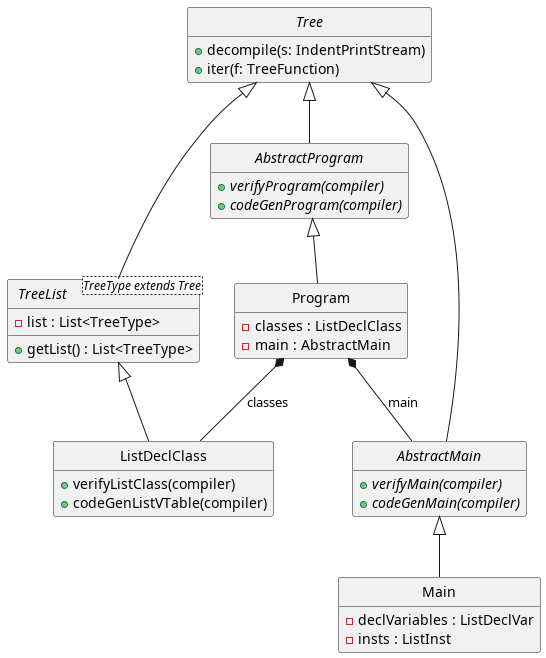
\includegraphics[width=0.5\textwidth]{diagrams/out/archi-ast-global.png}
    \caption{Structure de haut niveau de l'AST}
    \label{fig:ast-global}
\end{figure}

\noindent
Les points essentiels de cette correspondance sont les suivants :  
\begin{itemize}[label=$\circ$]
    \item Chaque terminal de la grammaire est représenté par une classe concrète, tandis que chaque non-terminal correspond à une classe abstraite dont héritent les classes concrètes appropriées.  
    \item Les ensembles de nœuds (listes de variables, méthodes, champs, paramètres) sont représentés par des classes héritant de \texttt{TreeList}, paramétrées sur le type des éléments. 
    \item L'héritage des classes reflète les relations dans la grammaire abstraite
    \item Chaque parcours de l'arbre (décompilation, vérification contextuelle, génération de code) correspond à une méthode abstraite déclarée dans la super-classe abstraite appropriée.
\end{itemize}

\noindent
Cette approche vise à minimiser les erreurs liées à un traitement au cas par cas, comme le ferait un code utilisant \texttt{instanceof} ou des tests sur les opérateurs, et facilite l'extension du compilateur avec de nouveaux types de nœuds.

\subsection{Lien entre l'AST et l'analyse contextuelle}
\noindent
Un objectif majeur auquel doit répondre l'architecture du compilateur est de distinguer la représentation syntaxique du programme de l'interprétation sémantique de ses éléments, tout en permettant l'interaction des deux. Les classes \texttt{DeclClass}, \texttt{DeclMethod}, \texttt{DeclField} et \texttt{DeclParam} sont instanciées par le parser lorsque des déclaration de la bonne forme sont reconnues dans le code source. Ce sont les nœuds de l'AST. 

\noindent
Le paquetage \texttt{context} dépend d'une hiérarchie de définitions centrée autour de la classe abstraite \texttt{Definition}. La spécialisation de \texttt{Definition} en \texttt{TypeDefinition} et \texttt{ExpDefinition} permet de distinguer clairement les entités relevant du système de types (comme les classes) de celles qui sont manipulables dans des expressions.


\noindent
Étant donné que la vérification contextuelle a aussi pour but de préparer l'AST pour la génération de code, la classe \texttt{ClassDefinition} encapsule non seulement les informations propres à une classe (nombre de champs, nombre de méthodes, super-classe), mais également son environnement de membres dans la classe \texttt{EnvironmentExp} (lié aux environnements des super-classes dans une liste chaînée). De même, les classes \texttt{MethodDefinition}, \texttt{FieldDefinition} et \texttt{ParamDefinition} peuvent stocker des index servant lors de la génération de code. Toutes ces relations sont illustrées dans la figure~\ref{fig:ast-class-context}. \\

\vspace{0.3cm}
\noindent
\textit{Remarque :} L'implémentation de \texttt{EnvironmentExp} repose sur une \texttt{HashMap} qui associe les symboles à leurs définitions. Ce choix garantit une complexité de recherche en O(1) en moyenne ce qui est souhaitable puisque la recherche de noms est l'opération la plus fréquente lors de la décoration de l'AST et il n'y a pas d'ordre particulier à respecter. L'unicité est assurée manuellement lors de l'insertion dans l'environnement (par \texttt{SymbolTable})

\begin{figure}[H]
    \centering
    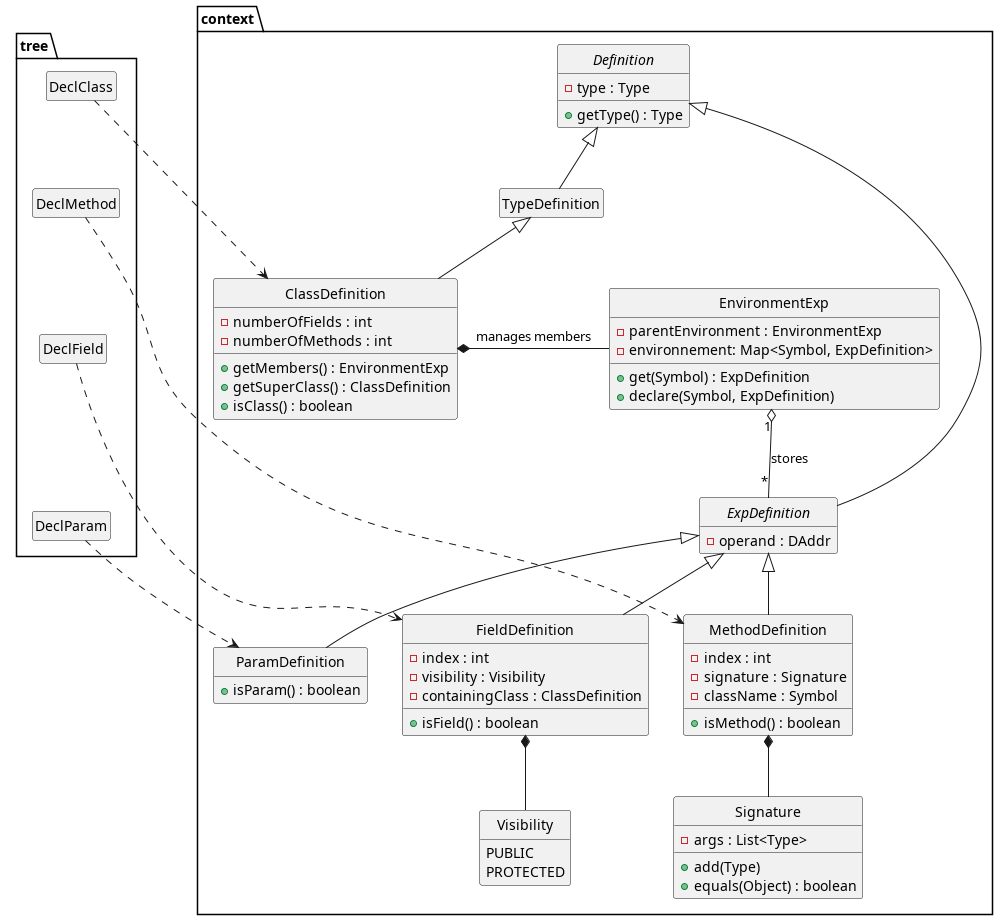
\includegraphics[width=0.8\textwidth]{diagrams/out/archi-class-context.png}
    \caption{Relations entre les nœuds de l'AST et les définitions contextuelles}
    \label{fig:ast-class-context}
\end{figure}

\noindent
Par exemple, lorsqu'une déclaration de méthode est rencontrée, une instance de \texttt{MethodDefinition} est créée et associée au nœud \texttt{DeclMethod} correspondant lors d'une passe de l'analyse contextuelle (\texttt{verifyMethodMembers}). Cette association permet d'ajouter à la déclaration le type de retour, ses paramètres et sa visibilité, des objets qui n'ont un sens qu'au moment de la vérification contextuelle.

\begin{code}[H]
    \lstinputlisting[style=Java,linerange={102-110}]{../../../src/main/java/fr/ensimag/deca/tree/DeclMethod.java}
    \caption{Extrait de la classe \texttt{DeclMethod} montrant l'association avec \texttt{MethodDefinition}}
    \label{code:decl-method}
\end{code}

\newpage
\noindent
L'analyse sémantique ne se limite pas aux structures de classes ; elle s'applique à chaque expression pour garantir la cohérence entre les types évalués et les types attendus. Comme l'illustre la figure~\ref{fig:ast-expr-context}, ce processus repose sur deux mécanismes :
\begin{itemize}[label=$\circ$]
    \item La décoration des nœuds : Chaque nœud héritant de \texttt{AbstractExpr} dispose d'un champ \texttt{type}. Lors de la vérification, ce champ est lié à l'une des instances uniques gérées par l'objet \texttt{EnvironmentType} (comme \texttt{INT} ou \texttt{FLOAT}), permettant des comparaisons de types efficaces par référence.
    \item La résolution des identificateurs : Contrairement aux littéraux qui portent leur type intrinsèquement, un \texttt{Identifier} doit interroger les environnements contextuels (\texttt{EnvironmentExp}) pour obtenir une \texttt{Definition}. Ce lien permet d'accéder aux métadonnées comme l'index en mémoire ou la visibilité d'un champ ou d'une méthode.
\end{itemize}

\begin{figure}[H]
    \centering
    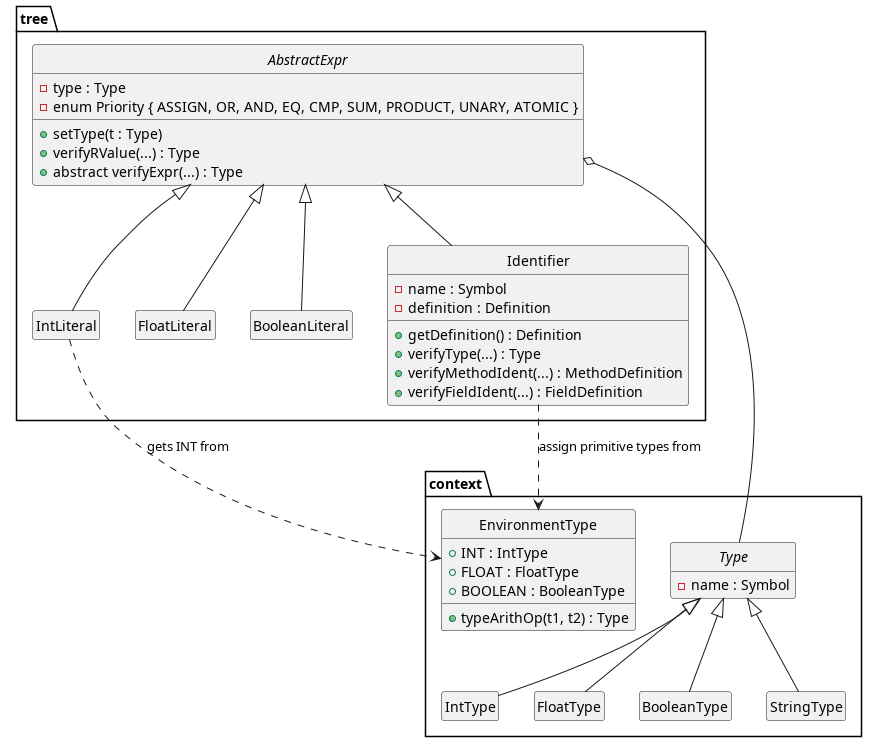
\includegraphics[width=0.8\textwidth]{diagrams/out/archi-expr-context.png}
    \caption{Relations entre les nœuds d'expression de l'AST et les définitions contextuelles}
    \label{fig:ast-expr-context}
\end{figure}

\noindent
Enfin, l'analyse contextuelle peut insérer un nœud \texttt{ConvFloat} : si une expression attend un flottant mais reçoit un entier, le compilateur encapsule le nœud original pour rendre la promotion explicite. Cette architecture pourrait permettre, par exemple, d'ajouter des transtypages implicites (comme une troncation d'entier) sans modifier la structure du compilateur existante, bien que ce type de comportement ne soit pas prévu dans le langage Deca.

\noindent
\textit{Remarque :} Le diagramme de la figure~\ref{fig:ast-expr-context} a été simplifié pour mettre en évidence les relations de décoration. L'attribut \texttt{Priority} de \texttt{AbstractExpr} est quant à lui utilisé lors de la phase de décompilation pour assurer une gestion correcte de la priorité des opérateurs lorsqu'il faut rajouter des parenthèses.
\subsection{Architecture de la génération de code} 
\noindent L'étape de génération de code transforme l'AST décoré en instructions pour la machine virtuelle \texttt{IMA}. Cette phase s'appuie sur une série de gestionnaires qui centralisent le code et en facilitent la maintenance. 

\subsubsection{Gestionnaires de ressources (Managers)}
\noindent Chaque gestionnaire est responsable d'un (ou plusieurs) aspect spécifique du processus de génération de code :

\begin{itemize}[label=$\to$]
    \item \texttt{VTableManager} et \texttt{VTableLayout} : Ces classes construisent la structure des tables des méthodes virtuelles. Elles prennent en charge l'héritage en copiant la table de la super-classe avant d'ajouter ou de mettre à jour les entrées pour les méthodes redéfinies. Le gestionnaire réserve également les slots nécessaires en base de pile globale (\texttt{GB}). Ce gestionnaire est aussi chargé de générer les instructions relatives à la classe \texttt{Object}
    \item \texttt{RuntimeErrorManager} : Afin d'optimiser la taille du code, ce gestionnaire centralise les types d'erreurs (\textit{division\_by\_zero}, \textit{null\_dereference}, \textit{heap\_overflow}, etc.). Il ne génère le bloc d'instructions \texttt{WSTR} et \texttt{ERROR} associé, qu'une seule fois en fin de fichier, et uniquement si une instruction susceptible de provoquer l'erreur a été rencontrée durant le parcours de l'AST.
    \item \texttt{LabelManager} : Il garantit l'unicité des étiquettes (\texttt{Label}) pour les structures de contrôle (\texttt{if}, \texttt{while}), les instructions \texttt{cast} et \texttt{instanceof}, ainsi que pour les méthodes et l'initialisation des champs. Chaque étiquette est suffixée d'un entier incrémenté par un compteur dédié, évitant ainsi toute collision de noms.
    \item \texttt{RegisterManager} : Ce gestionnaire contrôle l'utilisation des registres de la machine (\texttt{R2} à \texttt{R15}). Il fournit le prochain registre disponible en suivant un principe d'allocation séquentielle. Cette stratégie, s'appuyant sur un simple compteur (et non pas une structure de données complexe), est rendue possible par la structure récursive de l'AST qui garantit que les registres seront libérés dans l'ordre inverse de leur allocation. Le gestionnaire assure aussi le débordement (\textit{spilling}) : si tous les registres sont occupés, il génère automatiquement une instruction \texttt{PUSH} pour sauvegarder le contenu sur la pile, puis un \texttt{POP} pour le restaurer. Enfin, il gère la sauvegarde du contexte lors des appels de méthodes avec les méthodes \texttt{saveRegisters} et \texttt{restoreRegisters}.
    \item \texttt{StackManager} : Il suit l'occupation de la pile globale (\texttt{GB}) pour les variables globales et les tables des méthodes, ainsi que de la pile locale (\texttt{LB}) pour les variables locales et les paramètres. Il permet de calculer avec précision la taille maximale nécessaire à l'exécution du programme.
\end{itemize}

\subsubsection{Organisation du code généré}
\noindent
L'un des défis de la génération de code réside dans le fait que certaines informations, comme la taille totale de la pile, ne sont connues qu'une fois l'intégralité de l'AST parcourue. Pour résoudre ce problème sans effectuer de passes supplémentaires, le compilateur utilise plusieurs instances de \texttt{IMAProgram}. Le code est généré dans des blocs distincts (\texttt{head} pour les tables des méthodes, \texttt{body} pour le programme principal, et \texttt{preamble} pour les instructions de contrôle). Ces blocs sont concaténés dans l'ordre approprié par la classe \texttt{Program}. Un résumé de cette organisation est présenté dans la figure~\ref{fig:archi-managers}.

\begin{figure}[H]
    \centering
    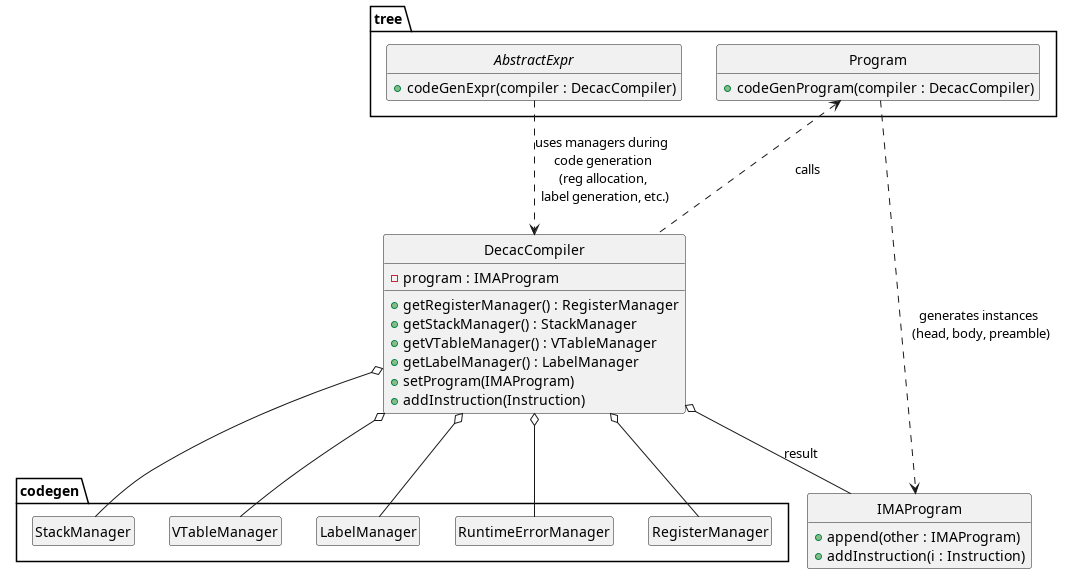
\includegraphics[width=0.9\textwidth]{diagrams/out/archi-managers.png}
    \caption{Architecture des gestionnaires de la génération de code}
    \label{fig:archi-managers}
\end{figure}

\subsubsection{Calcul de la taille de la pile et instructions d'initialisation}
\noindent
Le début du fichier assembleur doit impérativement contenir les instructions \texttt{TSTO} (\textit{Test Stack Overflow}) et \texttt{ADDSP} (\textit{Add Stack Pointer}) pour éviter des pertes de données ou des crashs imprévus. Grâce au compteur du \texttt{StackManager}, le compilateur récupère les dimensions finales de la pile. La valeur passée à \texttt{TSTO} doit anticiper le pire scénario d'occupation de la mémoire pour garantir un arrêt propre en cas de dépassement. Le calcul combine les données de plusieurs gestionnaires :
\[ \texttt{TSTO} = \texttt{StackSize} + \texttt{NbSavedRegs} + \texttt{MaxTempUsage} \]

\begin{itemize}[label=$\circ$]
    \item \texttt{StackSize} : Emplacements pour les variables globales et les VTables (géré par le \texttt{StackManager}).
    \item \texttt{NbSavedRegs} : Nombre maximal de registres sauvegardés lors des appels de méthodes (fourni par le \texttt{RegisterManager}).
    \item \texttt{MaxTempUsage} : Pic d'utilisation de la pile lors de l'évaluation d'expressions complexes ou du débordement de registres (calculé par le \texttt{RegisterManager}).
\end{itemize}

\noindent
Cette valeur est vérifiée par une instruction \texttt{BOV} (\textit{Branch on Overflow}) qui pointe vers une étiquette d'erreur d'exécution générée par le \texttt{RuntimeErrorManager}.

\section{Organisation de l'analyse contextuelle}
\noindent
L'analyse contextuelle est divisée en trois passes afin de résoudre les problèmes de {forward reference}. Ces différentes passent permettent de recenser les types avant leur utilisation comme types de champs ou de paramètres et de déclarer l'ensemble des membres (champs et méthodes) avant de vérifier la cohérence sémantique du corps des méthodes/classes.

\subsection{Conventions de nommage et traçabilité}
\noindent
Afin de maintenir une correspondance directe avec le polycopié de référence, nous avons ajouté dans la Javadoc de chaque méthode le numéro de la passe et la règle associée lorsque cela était pertinent. L'implémentation suit la convention de nommage suivante :
\begin{center}
    \texttt{verify[Nom\_de\_classe][Passe]}
\end{center}
\noindent
Les suffixes de passes ont été choisis pour refléter fidèlement la sémantique de l'étape :
\begin{itemize}[label=$\circ$]
    \item la Passe 1 identifie les classes et la hiérarchie 
    \item la Passe 2 (\texttt{Members}) vérifie les signatures des membres (champs et méthodes)
    \item la Passe 3 (\texttt{Body}) traite le code exécutable et les initialisations. Par souci de clarté, ces noms ont été adaptés lorsque le contexte l'exigeait (par exemple, on utilise \texttt{verifyFieldRValue} en passe 3 d'une déclaration de champ (\texttt{DeclField}), plutôt que \texttt{verifyBody}, qui n'avait pas beaucoup de sens).
\end{itemize}

\subsection{Synthèse des erreurs et vérifications}
\noindent
Conformément aux spécifications de [SyntaxeContextuelle] du polycopié, chaque règle de la grammaire attribuée impose des conditions dont le non-respect déclenche la levée d'une \texttt{ContextualError}. Le tableau ci-dessous recense les raisons de ces erreurs ainsi que les messages d'erreur associés.

\subsubsection{Passe 1 : Types et Hiérarchie}

\begin{center}
\renewcommand{\arraystretch}{1.5}
\begin{tabular}{|l|p{8cm}|p{6cm}|}
    \hline
    \rowcolor{gray!20} \textbf{Règle} & \textbf{Opération partielle / Condition} & \textbf{Message d'erreur} \\ \hline
    (1.3) & Nom de classe déjà présent dans \texttt{env\_types}. & Type <s> is already defined. \\ \hline
    (1.3) & Super-classe non trouvée dans l'environnement. & Superclass <name> of class <C> is not defined. \\ \hline
    (1.3) & La super-classe n'est pas de type \texttt{class}. & Superclass <name> is not a class type. \\ \hline
    (0.2) & Identificateur de type inconnu. & Type <name> not found \\ \hline
\end{tabular}
\end{center}

\subsubsection{Passe 2 : Déclarations des Membres (Champs et Méthodes)}

\begin{center}
\renewcommand{\arraystretch}{1.5}
\begin{tabular}{|l|p{8cm}|p{6cm}|}
    \hline
    \rowcolor{gray!20} \textbf{Règle} & \textbf{Opération partielle / Condition} & \textbf{Message d'erreur} \\ \hline
    (2.5) & Déclaration d'un champ de type \texttt{void}. & Field type cannot be void \\ \hline
    (2.5) & Nom de champ identique à une méthode héritée. & Field name collides with an inherited method \\ \hline
    (2.5) & Double déclaration d'un champ dans la même classe. & Field <name> already defined in class \\ \hline
    (2.7) & Méthode déjà définie dans la classe courante. & Method '<name>' is already defined in class '<C>'. \\ \hline
    (2.7) & Incompatibilité de signature ou type de retour (\textit{override}). & Method '<name>' has incompatible signature/type. \\ \hline
    (2.9) & Paramètre de méthode déclaré comme \texttt{void}. & Parameter cannot be of type void \\ \hline
    (2.9) & Double déclaration d'un paramètre. & Parameter <name> is already defined \\ \hline
\end{tabular}
\end{center}

\subsubsection{Passe 3 : Vérification des Corps et des Expressions}

\begin{center}
\renewcommand{\arraystretch}{1.5}
\begin{tabular}{|l|p{8cm}|p{6cm}|}
    \hline
    \rowcolor{gray!20} \textbf{Règle} & \textbf{Opération partielle / Condition} & \textbf{Message d'erreur} \\ \hline
    (3.17) & Variable locale déclarée avec le type \texttt{void}. & Variable type cannot be void \\ \hline
    (3.17) & Double déclaration d'une variable locale. & Variable <name> is already defined \\ \hline
    (3.22) & Condition de contrôle non booléenne. & Condition must be a boolean. Found: <type> \\ \hline
    (3.24) & Expression de \texttt{Return} de type \texttt{void}. & Return expression cannot be of void type \\ \hline
    (3.28) & Incompatibilité d'affectation (\texttt{assign\_compatible}). & Incompatible types in Rvalue... cannot assign <T1> to <T2> \\ \hline
    (3.31) & Paramètre de \texttt{print} invalide. & Invalid parameter type (expected int, float, or string) \\ \hline
    (3.33) & Types incompatibles pour une opération arithmétique. & Incompatible types for arithmetic operation \\ \hline
    (3.37) & \texttt{UnaryMinus} sur un type non numérique. & Operand of UnaryMinus must be of numeric type \\ \hline
    (3.39) & Échec de la compatibilité du \texttt{Cast}. & Cannot cast from <T1> to <T2> \\ \hline
    (3.42) & \texttt{New} utilisé sur un type non-classe. & New can only be used with class types \\ \hline
    (3.43) & \texttt{This} utilisé dans le \texttt{main} (hors classe). & 'this' cannot be used outside of a class \\ \hline
    (3.51) & Utilisation invalide du Modulo. & Incompatible types for modulo operation \\ \hline
    (3.63) & Opérateur \texttt{Not} sur un type non-booléen. & Operand of Not ('!') must be of boolean type \\ \hline
    (3.66) & Violation des droits d'accès au champ protégé. & Visibility error for protected field \\ \hline
    (3.67) & Identificateur inconnu dans l'environnement. & Identifier <name> not found \\ \hline
    (3.71) & Mauvais nombre d'arguments lors de l'appel. & Expected <n> args, got <m> \\ \hline
\end{tabular}
\end{center}

\section{Gestion et classification des erreurs}
\noindent
Le compilateur distingue plusieurs catégories d'erreurs, conformément aux spécifications fournies. Chaque étape de compilation possède son propre mécanisme de détection mais aussi ses propres erreurs (et exceptions) pour permettre de facilement identifier la source du problème lorsqu'une erreur survient.

\subsection{Erreurs dans un fichier \texttt{.deca}}
\noindent
Il s'agit des erreurs dues à un programme \texttt{.deca} incorrect, qui doit alors être rejeté par le compilateur. Ces erreurs peuvent être détectées à différentes étapes de la compilation (étapes A et B principalement). Dans ce cas, la compilation est immédiatement interrompue dès la première erreur détectée, sans tentative de récupération d'erreur.


\subsection{Erreurs internes}
\noindent
Les erreurs internes sont dûes à des défaillances du compilateur lui-même (bugs, mauvaises implémentations). Elles entraînent l'arrêt immédiat du compilateur, mais ne devraient pas se produire lors d'une utilisation normale.

\subsection{Signalement des erreurs}
\noindent
La détection et la propagation des erreurs reposent sur le mécanisme d'exceptions en Java, conformément aux instructions. Le compilateur s'arrête à la première erreur rencontrée.

\begin{itemize}[label=$\circ$]
    \item \texttt{RecognitionException} pour les erreurs de l'analyse syntaxique
    \item \texttt{ContextualError} pour les erreurs détectées lors de l'analyse contextuelle
    \item \texttt{CLIException} pour les erreurs liées à la ligne de commande
    \item \texttt{DecacFatalError} pour les erreurs d'entrée/sortie
    \item \texttt{DecacInternalError} pour les erreurs internes.
\end{itemize}

\noindent
Les messages d'erreur respectent le format imposé :
\begin{center}
\texttt{<nom-fichier>:<no-ligne>:<no-colonne>: <description>}
\end{center}

\noindent
\textit{Remarque: } Les avertissements n'ont pas été implémentés dans la version actuelle du compilateur. Un avertissement est affiché lorsqu'un programme \texttt{.deca} est correct mais pour lequel le compilateur détecte une situation éventuellement problématique. Dans ce cas le compilateur pourrait générer le code assembleur, mais signalerait le problème potentiel à l'utilisateur.trice par un message d'avertissement.

